\documentclass[[a4paper,11pt]{article}
\renewcommand{\rmdefault}{ptm}
\usepackage[scaled=0.92]{helvet}
\usepackage{courier,xcolor,colortbl,listings,parskip,graphicx,fancyvrb,fancyhdr,lastpage}
\usepackage{float,framed}
\normalfont
\usepackage[T1]{fontenc}
\setlength{\parskip}{7pt}
\usepackage[toc,page]{appendix}
\usepackage[hmargin=2.5cm,vmargin=2cm]{geometry}
\usepackage[utf8]{inputenc}
\usepackage[brazil]{babel}
\pagestyle{fancy}
\setlength{\headheight}{120pt}
\setlength{\headsep}{30pt}
\setlength{\textheight}{550pt}
\renewcommand{\headrulewidth}{0pt}
\lhead{}
\rhead{}
\chead{
\includegraphics{brasao.jpg}\\
        \large \textbf{PRESIDÊNCIA DA REPÚBLICA}\\
        \large SECRETARIA-GERAL\\
        \large Secretaria-Executiva}
\cfoot{}
\rfoot{\thepage /\pageref{LastPage}}
\hyphenation{par-ti-ci-pa-ção}
\bibliographystyle{ieeetr}

\newcommand{\MyName}{Daniela Soares Feitosa}
\newcommand{\MyEmail}{daniela@colivre.coop.br}
\newcommand{\ContractNumber}{2013/000292}
\newcommand{\ProjectCode}{Projeto PNUD BRA/12/018}
\newcommand{\NomeSecretaria}{Secretaria Geral da Presidência da República}
\newcommand{\SiglaSecretaria}{SG/PR}
\newcommand{\ProductNumber}{02}
\newcommand{\ProductDescription}{Documento com proposta para
desenvolvimento do código do tema padrão, painel de controle e
administração do portal contendo exemplos e códigos.}
\newcommand{\MesEntrega}{Novembro de 2013}
\newcommand{\DiaEntrega}{22}

\begin{document}
\lstset{language=Ruby}
\definecolor{light-gray}{gray}{0.95}
\lstdefinestyle{codeFrame}{backgroundcolor=\color{light-gray},frame=lines}

\textbf{\ProjectCode \ -} \ProductDescription

\vspace{3cm}

\begin{minipage}{0.5\textwidth}
  \textbf{Consultora: \MyName}
  \newline
  \textbf{Contrato nº: \ContractNumber}
  \newline
  \textbf{Produto / nº: \ProductNumber}
\end{minipage}

\vspace{2cm}

\textbf{Assinatura do Consultor}

\begin{framed}
Local e data: Brasília/DF, \line(1,0){20} \ de \line(1,0){100} \ de 2014
\newline
\newline
Assinatura do Consultor: \line(1,0){300}
\end{framed}

\vspace{1cm}

\textbf{Assinatura do Supervisor}

\begin{framed}
Atesto que os serviços foram prestados conforme estabelecido no Contrato
de Consultoria.
\newline
\newline
Local e data: Brasília/DF, \line(1,0){20} \ de \line(1,0){100} \ de 2014
\newline
\newline
Assinatura e Carimbo: \line(1,0){300}
\end{framed}

\clearpage
\newcolumntype{g}{>{\columncolor{light-gray}}l}

\begin{center}
  \begin{tabular}{| g | p{10cm} |}
    \hline
    \textbf{Título} & \ProductDescription \\ \hline
    \textbf{Língua do documento} & Português - Brasil \\ \hline
    \textbf{Documentação de referência} & Português \\ \hline
    \textbf{Unidade responsável} & \NomeSecretaria \
(\SiglaSecretaria) \\ \hline
    \textbf{Criador} & \MyName - \MyEmail \\ \hline
    \textbf{Taxonomias} & Desenvolvimento \\ \hline
    \textbf{Data de aprovação} &  \\ \hline
    \textbf{Público} & \SiglaSecretaria, Parceiros e Sociedade
Civil \\ \hline
    \textbf{Faz parte do} & \ProjectCode \\ \hline
    \textbf{Em conformidade com a} & \NomeSecretaria \\ \hline
    \textbf{Documentos anexos} & Página da Comunidade OSC - Organizações da
Sociedade Civil; CSS do cabeçalho do tema de comunidade; Código javascript para
incluir uma classe identificadora; Código CSS para estilizar os blocos com o padrão
colorido \\ \hline
    \textbf{Revisado em} &  \\ \hline
  \end{tabular}
\end{center}

\clearpage

\tableofcontents
\clearpage
\listoffigures

\clearpage

\section{Introdução}

A participação social no Brasil representa princípio
jurídico-institucional
presente na Constituição Federal de 1988, que a definiu como forma de
afirmação da
democracia e da consolidação da cidadania. Ao incorporar esse princípio
como
referência para a gestão pública, o Governo Federal aprimora os
processos de interação
do Estado com a sociedade e cria as condições institucionais para a
prática da
democracia participativa. Com isso, verifica-se que, além da crescente
participação
social nas decisões governamentais, as políticas públicas ganham maior
legitimidade,
uma vez que expressam as atuais condições socioeconômicas e culturais da
população
brasileira em suas diferentes realidades regionais.

Na estrutura administrativa do Poder Executivo Federal, cabe à
Secretaria-Geral
da Presidência da República (SG/PR) a função de intermediar as relações
do Governo
com as entidades da sociedade civil, conforme competências definidas
pela Lei
10.683/2003 e pelo Decreto no. 7.688/2012. Assim, a SG/PR é órgão
incumbido de
assessorar diretamente a Presidenta da República e os órgãos e entidades
do Governo
Federal no relacionamento e na articulação com os movimentos sociais, o
que inclui a
criação e a implementação de canais que assegurem a consulta e a
participação popular
na discussão e na definição da agenda prioritária do país.

O Brasil tem um rico histórico de efetivação da democracia
participativa, sendo
reconhecido mundialmente. Os instrumentos institucionalizados como
conselhos de
políticas públicas e conferências nacionais foram profundamente
ampliados na última
década, contando com um legado volumoso de práticas e realizações. A
maioria dos
programas de governo já conta com participação social prevista em pelo
menos uma de
suas etapas. As práticas trazidas pelas novas mídias e pela cultura
digital podem
interagir nesses espaços fortalecendo, ampliando e aprofundando a
democracia
participativa, já na abordagem do novo século, pós redes sociais
digitais.

Incentivando os atores a conectar perfis, blogs e demais instâncias de
produção
de conteúdo na rede, o Portal de Participação Social poderá se
estabelecer como um
repositório agregador do conhecimento sobre participação social hoje
disperso na
internet e nas instâncias governamentais. A partir de uma interface
clara que possibilite
a navegação pelos temas, o Portal de Participação Social pode ser um
espaço onde os
diferentes agentes de governo, movimentos, organizações e cidadãos em
geral
encontrarão solo fértil e facilitado para o exercício da pesquisa e do
diálogo.

Tendo por base a premissa de que a incursão e abertura de canais de
acesso ao
poder público na rede aumenta o conhecimento das ações do governo e
diminui as
barreiras para participação de cidadãos, entidades e movimentos, esse
projeto visa a
construção de um conjunto de ferramentas que poderão ser utilizadas por
gestores e
servidores para proporcionar novas formas de participação a serem
apropriadas pela
cidadania. Além disso, esse portal também buscará dar evidência às
formas de
participação existentes no sentido de contextualizar, organizar e
facilitar o acesso do
cidadão às formas de incidir nas diversas etapas das políticas públicas
do governo
brasileiro.

\section{Apresentação}

Este documento é parte da consultoria para o projeto
\textbf{Desenvolvimento de Metodologias de Articulação e Gestão de
Políticas Públicas para Promoção da Democracia Participativa}
(BRA/12/018), firmado entre a Secretaria-Geral da Presidência da República
(SG/PR) e o Programa das Nações Unidas para o Desenvolvimento (PNUD).
A consultoria tem como objetivo a especificação da construção dos códigos das
metodologias de organização da informação e interação participativa do
portal da participação social.

O presente documento apresenta a proposta para
desenvolvimento do código do tema padrão, painel de controle e
administração do portal contendo exemplos e códigos. 
Essa proposta está configurada como produto 2 da consultoria técnica.

Neste documento será apresentada a especificação e
modelagem para desenvolvimento do código necessário para aplicação do
tema padrão como definido pela equipe do projeto.

O Portal de Consulta Pública utiliza o software livre Noosfero,
plataforma web para redes sociais, então o código produzido deverá ser público
e divulgado para a comunidade e para os que desenvolvem e se utilizam do
software.

Como conteúdo deste documento também serão apresentados as propostas de
código para adaptação do Noosfero e especificação do CSS para adequação
ao tema aprovado.

\section{Tema padrão do Portal de Consulta Pública}

As ideias que serviram como base para a definição da arquitetura de
informação e do tema padrão do portal de Consulta Pública foram
discutidas em reuniões com integrantes da Secretaria Geral da
Presidência da República (SG/PR), Parceiros e Sociedade Civil.

O gráfico do layout para a rede social
/portal foi desenvolvido por Fabiano Rangel, consultor do projeto
BRA/12/018, e aprovado pela equipe gestora do projeto. O tema padrão
pode ser visualizado no
Anexo~\ref{Att:PaginaInicial}.

Como o Noosfero não possui os recursos necessários para que o tema seja
aplicado, será necessário o desenvolvimento do código. Nas subseções
seguintes, serão
detalhados a modelagem dos códigos necessários para os elementos da
página.

\subsection{Barra de Identidade do Governo Federal na Internet}

\begin{figure}[h]
\center
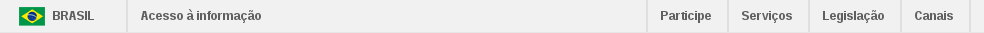
\includegraphics[scale=0.5]{barra-governo.png}
\caption{Barra de Identidade}
\label{fig:barra-governo}
\end{figure}

A barra de identidade do Governo Federal na internet
(Figura~\ref{fig:barra-governo}) tem a função de identificar, padronizar
e integrar sítios e
portais do Governo Federal. À sua esquerda constam as marcas do Governo
Federal e da Lei de Acesso à Informação com links para acesso ao Portal
de Estado do Brasil www.brasil.gov.br e o sítio oficial sobre acesso à
informação www.acessoainformacao.gov.br. À sua direita constam outros
links de grande relevância aos cidadãos.

O Portal de Participação Social também implementa a barra, que deverá
ser mantida mesmo em perfis que tenham layout próprio.

Seu uso está normatizado por meio da Instrução Normativa nº 2, de 16 de
dezembro de 2009, que pode ser encontrada no sítio da Secretaria de
Comunicação Social da Presidência da República - Secom. Seguindo as
orientações, o código abaixo deverá ser incluído no tema no Portal e em
todos os temas aplicados nos perfis.

{\scriptsize
  \begin{verbatim}
  <div id="barra-brasil">
      <a href="http://brasil.gov.br" style="background:#7F7F7F; height:
  20px; padding:4px 0 4px 10px; display: block;
  font-family:sans,sans-serif; text-decoration:none; color:white; ">Portal
  do Governo Brasileiro</a>
  </div>
  <script src="http://barra.brasil.gov.br/barra.js"
  type="text/javascript"></script>
  \end{verbatim}
}

\subsection{Cabeçalho do Portal de Participação}

\begin{figure}[h]
\center
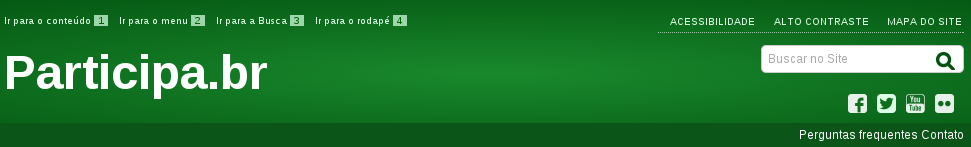
\includegraphics[scale=0.5]{cabecalho-portal.png}
\caption{Cabeçalho do portal}
\label{fig:cabecalho-portal}
\end{figure}

O cabeçalho do Portal de Participação Social do Governo Federal na internet
(Figura~\ref{fig:cabecalho-portal}) segue o modelo utilizados
em outros sites do Governo Federal.

À esquerda constam os links para acesso rápido à algumas
seções da página e o nome do Portal.
À direita constam os links de acessibilidade, mapa do site, campo de
busca, links para outras redes sociais e links de perguntas e contato do
Portal.

O código que gera o cabeçalho do Portal pode ser visualizado no
Anexo~\ref{Att:CabecalhoPortal}.

\subsection{Barra de Participação Social}

\begin{figure}[h]
\center

\includegraphics[scale=0.5]{barra-participa.png}
\caption{Barra de Participação Social}
\label{fig:barra-participacao}
\end{figure}

Na barra de participação social (Figura~\ref{fig:barra-participacao}) serão
mostradas as categorias
cadastradas no portal. Cada categoria será um link para uma tela que
mostrará todas as trilhas cadastradas na categoria.

Essa barra também poderá ser incorporada em outros sites e portais,
possibilitando uma maior integração e participação nas consultas
públicas.
Para essa incorporação, o Noosfero deverá ter uma interface que
disponibilizará as informações sobre as categorias do portal.

Para a implementação da barra foi desenvolvido o código abaixo, que
lista as categorias disponíveis no ambiente com a cor definida pelo
administrador.

{\scriptsize
  \begin{verbatim}
  <ul id="cat_menu">
    <% @environment.display_categories.each do |item| %>
      <li id="category<%= item.display_color %>">
        <%= item.name %>
      </li>
    <% end %>
  </ul><!-- fim id="cat_menu" -->
  \end{verbatim}
}

Para que a barra seja incorporada em outros sites/portais, será
disponibilizado um endereço
público que ainda será definido, como {\it
http://participa.gov.br/barra.js}, que obterá as informações
sobre as categorias e deverá ser colado no html do
site/portal,
seguindo o mesmo padrão utilizado na barra do Governo Federal:

{\scriptsize
  \begin{verbatim}
  <div id="barra-participacao">
      <a href="http://participa.gov.br">Portal de Participação
  Social do Governo Brasileiro</a>
  </div>
  <script src="http://participa.gov.br/barra.js"
  type="text/javascript"></script>
  \end{verbatim}
}

Para garantir a identidade visual da barra, o endereço público
deverá conter também o CSS da barra. Além disso, será necessário
definir as
normas de aplicação e instruções sobre o uso da barra no portal de
Participação Social.

\subsection{Bloco de Categorias com Relevância}

\begin{figure}[h]
\center
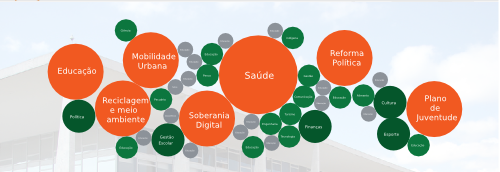
\includegraphics[scale=0.4]{bloco-categorias-bolas.png}
\caption{Bloco de categorias}
\label{fig:bloco-categorias-bolas}
\end{figure}

Todo o conteúdo criado no Portal de Participação Social pode ser
categorizado. As categorias são definidas pelo administrador do
ambiente. Com o objetivo de dar destaque às categorias com maior
relevância, será necessário criar um bloco como mostrado na
Figura~\ref{fig:bloco-categorias-bolas}.

Os critérios para definição da relevância de cada categoria ainda
precisam ser definidos. Alguma opções são:

\begin{itemize}
  \item Quantidade de conteúdo criado e classificados com a categoria;
  \item Número de comentários de usuários, que indicam a participação dos usuários, em
conteúdos com determinada categoria;
  \item Uma combinação dos critérios acima;
\end{itemize}

Considerando que no lançamento do portal não teria conteúdo suficiente
para indicar diferenças na relevância das categorias e a falta da
definição de quais seriam os critérios, para o lançamento foi criado um
bloco de {\it html}. Nesse bloco foi incluído o código
(Anexo~\ref{Att:CategoriasBolas}) que mostra as
categorias definidas pelos gestores como mais importantes e gera as bolas
de diferentes tamanhos e cores. Cada categoria/bola será um link para uma tela que
mostrará todas as trilhas cadastradas na categoria.

\subsection{Bloco de Estatísticas}

O Noosfero já possui um bloco de estatísticas que mostra a quantidade de
usuários e comunidades do ambiente. Como essas informações não são
suficientes para atender ao proposto pelo tema do portal
(Figura~\ref{fig:bloco-estatisticas}), o bloco de
estatísticas deverá ser alterado.

\begin{figure}[h]
\center
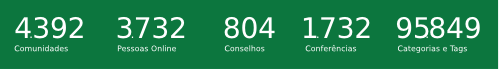
\includegraphics[scale=0.4]{bloco-estatisticas.png}
\caption{Bloco de estatísticas}
\label{fig:bloco-estatisticas}
\end{figure}

Para facilitar a incorporação do código desenvolvido no código oficial
do Noosfero, o bloco será migrado para ser utilizado como plugin e
deverá ser alterado para dar suporte à
personalização do bloco.

Na tela de edição do bloco, o administrador poderá escolher quais
informações serão visualizadas
(Figura~\ref{fig:bloco-estatisticas-edicao}).

\begin{figure}[h]
\center
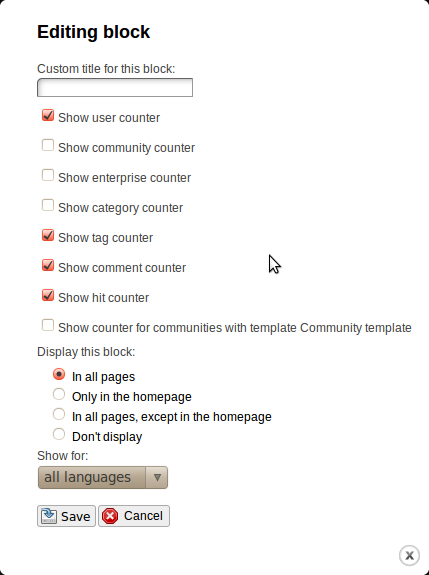
\includegraphics[scale=0.4]{bloco-estatisticas-edicao.png}
\caption{Edição do bloco de estatísticas}
\label{fig:bloco-estatisticas-edicao}
\end{figure}

\subsection{Bloco de Notícia Destaque}

O Noosfero já possui um bloco que mostra um determinado conteúdo, é o
plugin {\it DisplayContentPlugin}. Para atender ao proposto pelo tema do portal
(Figura~\ref{fig:bloco-noticia-destaque}), apenas será necessário que
seja desenvolvido o código CSS para estilizar o bloco.

\begin{figure}[h]
\center
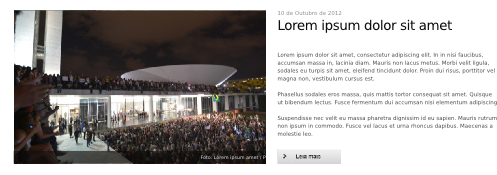
\includegraphics[scale=0.4]{bloco-noticia-destaque.png}
\caption{Bloco de notícia destaque}
\label{fig:bloco-noticia-destaque}
\end{figure}

\subsection{Bloco de Trilhas}

\begin{figure}[h]
\center
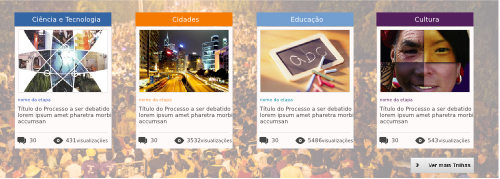
\includegraphics[scale=0.4]{bloco-trilhas.png}
\caption{Bloco de trilhas}
\label{fig:bloco-trilhas}
\end{figure}

O conceito de trilhas ({\it Tracks}) no Portal de Participação Social foi definido pela
equipe do projeto. As trilhas funcionam como forma de organização dos
elementos para discussão de determinado tema em uma comunidade. Cada trilha possui uma
descrição, objetivo, resultados esperados e é formado por passos ({\it
steps}).

Para utilização desse conceito no Noosfero, foi criado um novo tipo de
conteúdo que está disponível apenas para os perfis do tipo comunidade.
Seguindo a ideia de reaproveitamento de código e orientação a objetos,
esse novo tipo de conteúdo herda as informações de um tipo já presente
no Noosfero, o tipo {\it Folder}. As trilhas serão mostradas em um bloco
na página inicial, como mostrado na
Figura~\ref{fig:bloco-trilhas}.

Na criação da trilha, o usuário deverá definir o nome, descrição,
objetivos, resultados esperados e categoria. Além disso, poderá definir
os passos necessários para que a trilha seja percorrida. Cada passo
poderá ter uma ferramenta para participação. Inicialmente, para o
lançamento do portal, as ferramentas disponíveis serão artigos do tipo 
{\it TinyMceArticle} ou {\it Forum} e deverá ter data de início e fim.
Dessa forma, cada administrador poderá criar trilhas em suas
comunidades e definir os prazos para que cada passo seja realizado.

{\scriptsize
  \begin{verbatim}
  class CommunityTrackPlugin::Track < Folder                   
                                                               
    settings_items :goals, :type => :string                    
    settings_items :expected_results, :type => :string         
                                                               
    def self.icon_name(article = nil)                          
      'community-track'                                        
    end                                                        
                                                               
    def self.short_description                                 
      _("Track")                                               
    end                                                        
                                                               
    def self.description                                       
      _('Defines a track.')                                    
    end
  \end{verbatim}
}

\subsection{Blocos de Notícias da Capa}

\begin{figure}[h]
\center
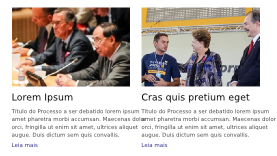
\includegraphics[scale=0.4]{bloco-destaques-menor.png}
\caption{Blocos de notícia da capa}
\label{fig:bloco-destaques-menor}
\end{figure}

Além da notícia de destaque, serão mostradas mais duas notícias na
página inicial do ambiente. Essas notícias serão inseridas no mesmo tipo
de bloco utilizado no outro bloco de destaque (mencionado acima). É o 
plugin {\it DisplayContentPlugin}. Para atender ao proposto pelo tema do portal
(Figura~\ref{fig:bloco-destaques-menor}), apenas será necessário que
seja desenvolvido o código CSS para estilizar o bloco.

\subsection{Bloco de Membros}

\begin{figure}[h]
\center
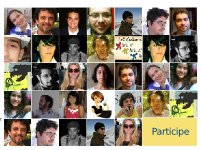
\includegraphics[scale=0.4]{bloco-integrantes.png}
\caption{Bloco de membros}
\label{fig:bloco-integrantes}
\end{figure}

O Noosfero já possui um bloco de membros que mostra as imagens dos
perfis dos usuários cadastrados no ambiente. A quantidade de usuários
que serão mostrados é definida na edição do bloco. Para atender ao
proposto pelo tema do portal (Figura~\ref{fig:bloco-integrantes}), o bloco de
membros deverá ser alterado para permitir que o administrado informe se
deseja que o botão de entrar ou sair da comunidade fique disponível.
Para facilitar a incorporação do código no código oficial do Noosfero,
por padrão esse botão não será mostrado.

Além da alteração no código do bloco, também será necessária a alteração
no CSS do bloco.

\subsection{Bloco de Mapa}

\begin{figure}[h]
\center
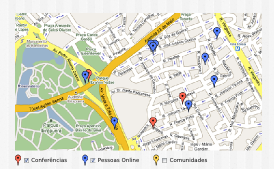
\includegraphics[scale=0.4]{bloco-mapa.png}
\caption{Bloco de mapa}
\label{fig:bloco-mapa}
\end{figure}

O bloco de mapa do ambiente (Figura~\ref{fig:bloco-mapa}) tem o objetivo de mostrar para os usuários
visitantes do site a geolocalização dos perfis cadastrados no ambiente.
Dessa forma, os usuários poderão verificar quais pessoas/comunidades
estão próximas ao usuário e onde as conferências serão realizadas.

No Noosfero todos tipos de perfis podem ser geolocalizados, já que podem
armazenar as coordenadas de latitude e longitude. No entanto, o mapa de localização
já existente no Noosfero só pode ser utilizado no contexto de perfis,
mas não de ambiente. Todo o conteúdo criado no Portal de Participação Social poderá ser
geolocalizado. 

Para o lançamento do portal foi criado um
bloco de {\it html}. Nesse bloco foi incluído o código que mostra um
mapa:

{\scriptsize
  \begin{verbatim}
  <iframe width="525" height="300" frameborder="0" scrolling="no"
  marginheight="0" marginwidth="0"
  src="https://maps.google.com.br/?ie=UTF8&amp;t=m&amp;ll=-12.744005,
  -38.616691&amp;spn=0.001831,0.00228&amp;z=18&amp;output=embed"></iframe>
  \end{verbatim}
}

Para atender ao proposto pelo tema do Portal, será necessário que o
bloco de localização seja alterado. Deverá ser possível que ele seja
adicionado no contexto de ambiente e que a localização dos perfis
cadastrados fiquem disponíveis.

\subsection{Bloco de Comunidades}

\begin{figure}[h]
\center
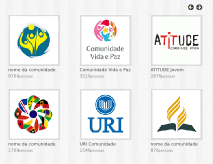
\includegraphics[scale=0.4]{bloco-comunidades.png}
\caption{Bloco de comunidades}
\label{fig:bloco-comunidades}
\end{figure}

O Noosfero já possui um bloco de comunidades que mostra as imagens das
comunidades cadastrados no ambiente. A quantidade de comunidades
mostradas é definida na edição do bloco. Para atender ao
proposto pelo tema do portal (Figura~\ref{fig:bloco-comunidades}), será
necessária apenas a alteração no CSS do bloco de comunidades.

\subsection{Bloco de Tags}

\begin{figure}[h]
\center
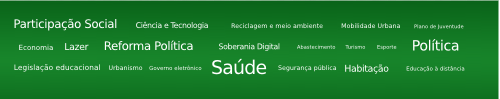
\includegraphics[scale=0.4]{bloco-tags.png}
\caption{Bloco de tags}
\label{fig:bloco-tags}
\end{figure}

O Noosfero já possui um bloco de {\it tags} que mostra as tags
utilizadas nos conteúdos do ambiente. A quantidade de
palavras/frases/expressões mostradas é definida na edição do bloco. Para atender ao
proposto pelo tema do portal (Figura~\ref{fig:bloco-tags}), será
necessária apenas a alteração no CSS do bloco de tags.

\subsection{Bloco de Vídeos}

\begin{figure}[h]
\center
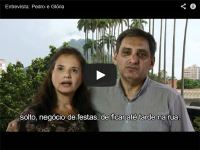
\includegraphics[scale=0.4]{bloco-video.png}
\caption{Bloco de vídeo}
\label{fig:bloco-video}
\end{figure}

O bloco de vídeos (Figura~\ref{fig:bloco-video}) tem o objetivo de
publicar vídeos ou streamming e poderá ser incluído no contexto de
perfil ou ambiente. 

Os vídeos suportados são os originados do youtube e vimeo e outros
formatos de vídeo, como mp4, ogg, ogv e webm.
Na tela de edição do bloco, o administrador do perfil ou ambiente poderá
definir o endereço e as dimensões do vídeo na página 
(Figura~\ref{fig:bloco-video-edicao}).

\begin{figure}[h]
\center
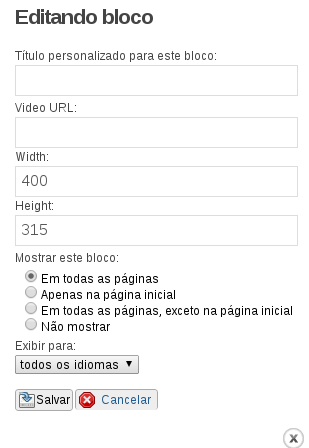
\includegraphics[scale=0.4]{bloco-video-edicao.png}
\caption{Edição do bloco de vídeo}
\label{fig:bloco-video-edicao}
\end{figure}

Para facilitar a incorporação do código desenvolvido no código oficial
do Noosfero, o bloco foi criado como plugin. Parte do código pode ser
visto abaixo:

{\scriptsize
  \begin{verbatim}
  class VideoBlock < Block
  
    settings_items :url, :type => :string, :default => ""
    settings_items :width, :type => :integer, :default => 400
    settings_items :height, :type => :integer, :default => 315
  
    def is_youtube?
      url.match(/.*(youtube.com.*v=[[:alnum:]]+|youtu.be\/[[:alnum:]]+).*/)
  ? true : false
    end
  
    def is_vimeo?
      url.match(/^(http[s]?:\/\/)?(www.)?(vimeo.com|player.vimeo.com\/video)\/[[:digit:]]+/)
  ? true : false
    end
  
    def is_video_file?
      url.match(/.*(mp4|ogg|ogv|webm)$/) ? true : false
    end
  end
  \end{verbatim}
}

\subsection{Folha de Estilo - CSS}

O CSS é utilizada para definir a apresentação de documentos escritos em
uma linguagem de marcação, como HTML ou XML. Seu principal benefício é
prover a separação entre o formato e o conteúdo de um documento.

Ao invés de inserir a formatação diretamente no documento, é inserido
um link na página para o arquivo que contém as definições de estilo.

A primeira versão do CSS pode ser visualizada no
Anexo~\ref{Att:CSS}. Essa versão foi a base para o
desenvolvimento de todo o estilo do Portal.

Essa primeira versão já adapta o tema padrão do Noosfero para o padrão
do Portal em todas as telas existentes (página inicial do ambiente e
perfis, tela de administração, painel de controle) antes do desenvolvimento dos
códigos descritos nesse documento.

Como o Portal estará sempre em evolução, o arquivo com o CSS do
portal deverá ser sempre atualizado para que os novos elementos
inseridos nas páginas sigam o padrão do tema do Portal.

\newpage

\section{Considerações finais}

Neste documento foram apresentados a especificação e modelagem
dos
códigos necessários para que o tema definido para o Portal de Consulta
Pública seja implementado no Noosfero. Além de código CSS, será
necessário o desenvolvimento de novos elementos e adaptação dos
já existentes na plataforma.

Deve ser considerado que tanto os itens
desenvolvidos para o Portal como os já existentes no Noosfero
poderão sofrer alterações com o objetivo de melhorar a
funcionalidade, usabilidade ou apresentação.

\vspace{1cm}

Sem mais nada a acrescentar, coloco-me à disposição.

\vspace{1cm}

\begin{minipage}{\textwidth}
  Brasília/DF, \DiaEntrega \ de \MesEntrega\\[1cm]
  \textbf{\MyName}\\
  \small Consultora do PNUD
\end{minipage}

\newpage
\appendix
\appendixpage
\section{Plugin class} \label{App:PluginCode}





\end{document}
